
\usepackage{float}
\addcontentsline{toc}{chapter}{Chapitre 3 : Introduction générale} 
\section{Introduction:}
Nous allons, dans ce chapitre, analyser et détailler le premier Sprint qui a pour but de réaliser la partie Authentification et la  sécurité . Ainsi que les différents stories. En premier lieu, nous présentons le backlog du Sprint
contenant l’ensemble des tâches à réaliser. Ensuite, nous allons raffiner les besoins et entamer la solution conceptuelle en exposant les différents diagrammes qui décrivent l’interactionentre le système et l’utilisateur afin d’atteindre le résultat désiré.
\section{Backlog Sprint1 }
Ce tableau représente le premier module du premier Sprint ainsi que les différents User Story.








\begin{table*}[h]
    \begin{center} 
    \begin{tabular}{|p{3cm}|p{5cm}|p{3cm}|p{1.9cm}|p{2cm}|} \hline 
          Module &  User Stories &  Tache &  Complexité & Estimation \\ \hline

            Gestion d'accé de la plateforme & En tant que visiteur je veux m'inscrire   & - Dévelopement du backend & \centering L & 1 jour  \\  \hline

            & En tant que étudiant je veux m’authentifier & & \centering L & 1 jour   \\ \hline
            & En tant que professeur je veux m'authentifer mon compte& & \centering  L & 1 jour   \\ \hline
            & En tant que admin je veux m'authentifier & & \centering  L & 1 jour   \\ \hline
           




       
    \end{tabular}
  \end{center}
  \center
  \caption { Backlog sprint1}
\label{tab:bert_res}
\end{table*}  




\section{Analyse fonctionnelle}
Dans cette partie on va présenter les besoins fonctionnels qui seront répartis suivant 2 modules à savoir :



\begin{itemize}
    \item \textbf{S'authetifier:} l'utilisateur va s'authentifier au plateforme après entrer ses coordonnés corrects.

    \item \textbf{S'inscrire}  : l'utilisateur va créer un compte pour accéder aux services et fonctionnalités après fournir les informations nécessaires qui sont "username" "email" et "password".


    

   
\end{itemize}
\section{Raffinement du sprint 1}
\subsection{Rafinnement de cas d'utilisation "Authentification"}
L’authentification est le besoin primordial pour le traitement et la sécurité des autres cas d’utilisation.
Pour que les utlisateurs qui sont un collaborateur, un formateur ou un admin  puissent exécuter leurs propres besoins, ils sont obligés de passer par l’authentification.
cette figure nous illustre le diagramme de cas d’utilisation « S’authentifier » :


\begin{figure}[!h]
\center
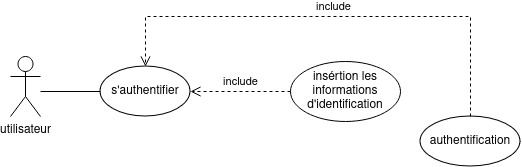
\includegraphics[width=0.8\textwidth]{pages/image/asma-usecase-authenthification.jpg}
\caption{Présentation de cas d'utilisation"s'authentifier"}
\end{figure}


\subsubsection{Déscription textuelle}  

\begin{table*}[h]
    \begin{center} 
    \begin{tabular}{|p{4cm}|p{9cm}|}  \hline 
       Cas d'utilisation& Authentification \\ \hline
       Acteur&collaborateur, formateur, admin \\ \hline
       Précondition&  L’utilisateur doit être enregistré dans la base
       de données      \\ \hline
       Post condition& L’utilisateur peut accéder aux différentes fonctionnalités du plateforme \\ \hline
       Scénario nominale&Le système affiche le formulaire d’identification. \\
       &L'utilisateur entre ses informations nécessaire pour s'authentifier.\\
          & Le systéme verifie les informations saisie par l'utilisateur et l'envoie vers la page d'acceuil .\\ \hline
       Scénario alternatif&      
        L'utilisateur saisie des données inncorrecte \\
         & L'utilisateur n'est pas enregistré au base de donnés \\
         & Un probléme de connexion.
          
     \\ \hline
  \end{tabular}
  \end{center}

  \caption{ Déroulement de cas d'utilisation d'authentification}
\label{tab:bert_res}
\end{table*}



















\subsection{Rafinnement de cas d'utilisation "S'inscrire"}
La figure 19 nous illustre le diagramme de cas d’utilisation « S’inscrire » :

\begin{figure}[!h]
\center%
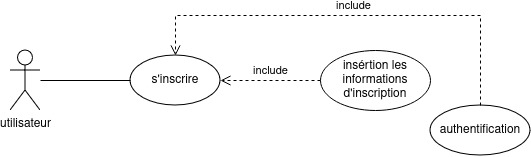
\includegraphics[width=0.8\textwidth]{pages/image/asma-usecase-inscrire.jpg}
\caption{Diagramme du cas d'utilisation "Inscrire"}
\end{figure}


\subsubsection{Déscription textuelle}  

\begin{table*}[h]
    \begin{center} 
    \begin{tabular}{|p{4cm}|p{9cm}|}  \hline 
       Cas d'utilisation& Inscrire \\ \hline
       Acteur&Visiteur,Etudiant,Admin,professeur \\ \hline
       Précondition& Connexion à l'internet   
       \\ \hline
       Post condition& L’utilisateur peut accéder aux différentes fonctionnalités du plateforme
       \\ \hline


       
       Scénario nominale& 
            L'utilisateur accéde à la page d'identification et fait l'inscription.\\
          &L'utilisateur entre ses informations nécessaire pour s'inscrire.\\
          & Le systéme verifie les informations saisie par l'utilisateur et l'envoie vers la page d'acceuil .
                       \\ \hline
                       
       Scénario alternatif&      
        L'utilisateur saisie des données inncorrecte \\
         & L'utilisateur n'est pas enregistré au base de donnés \\
         & Un probléme de connexion.
          
     \\ \hline
  \end{tabular}
  \caption{Déroulement de cas d'utilisation}
  \end{center}
\label{tab:bert_res}
\end{table*}













\section{Conception}
\subsection{Diagramme de classe  }
La figure suivant montre le diagramme de classe pour la procedure d'authentification: 
\begin{figure}[h]
    \centering
    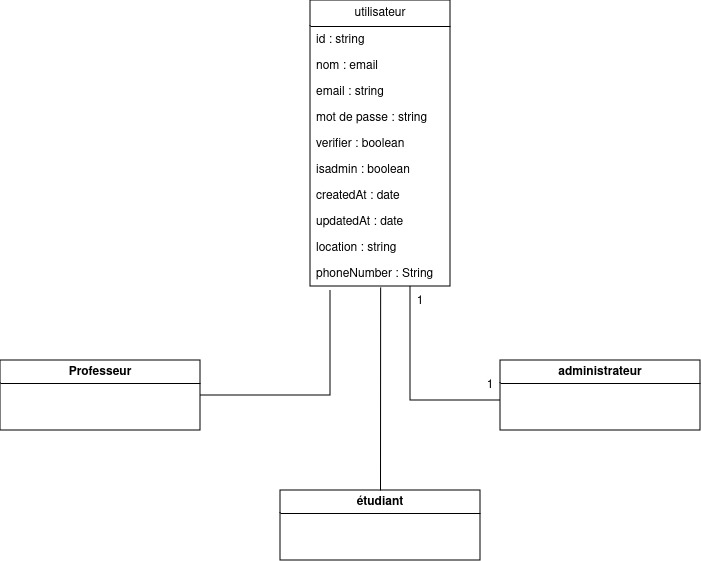
\includegraphics[width=0.65\linewidth]{pages/image/asma-class_diagramme-authentifier.jpg}
    \caption{Diagramme de classe "authentification"}
    \label{fig:enter-label}
\end{figure}

La figure suivant montre le diagramme de classe pour la procedure d'authentification: 

\begin{figure}[h!]
    \center
    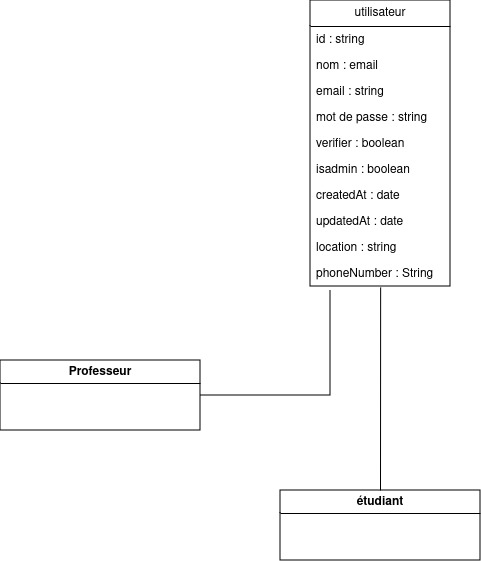
\includegraphics[width=0.5\linewidth]{pages/image/asma-classdiagramme-inscrire.jpg}
    \caption{Diagramme de classe "inscription"}
\end{figure}







\subsection{Diagramme de séquance :}
\subsubsection{Conception de partie "Authentification"}
Cette figure représente le diagramme de séquance pour l'authentification d'un utilisateur de la plateforme .\\
\begin{figure}[h!]
\center
  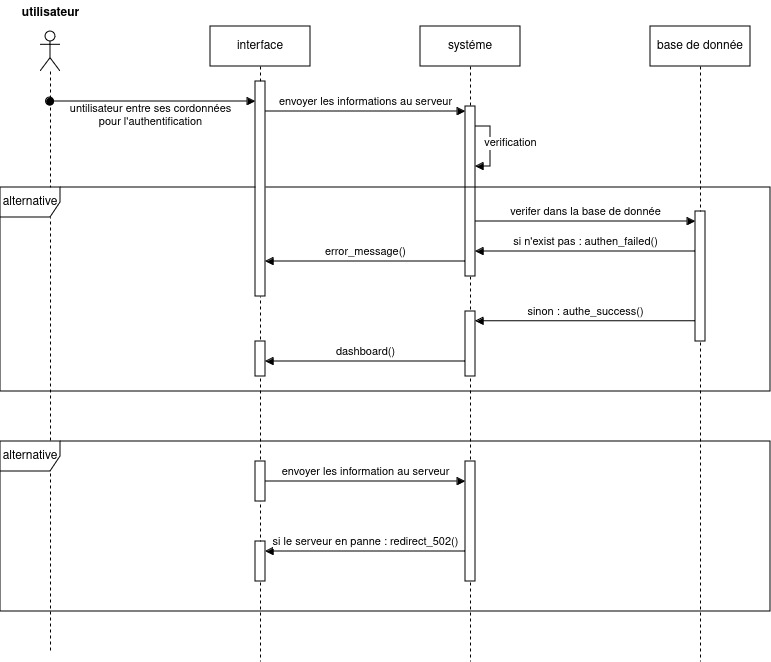
\includegraphics[width=0.6\linewidth]{pages/image/asma-diagramme_sequence-authentification.jpg}
    \caption{Diagramme de séquance  pour l'authentification d'un etudiant}
    \label{fig:enter-label}
\end{figure}




















Cette figure représente le diagramme de séquance pour l'inscription de l'utilisateur au plateforme .\\
\begin{figure}[h!]
\center
  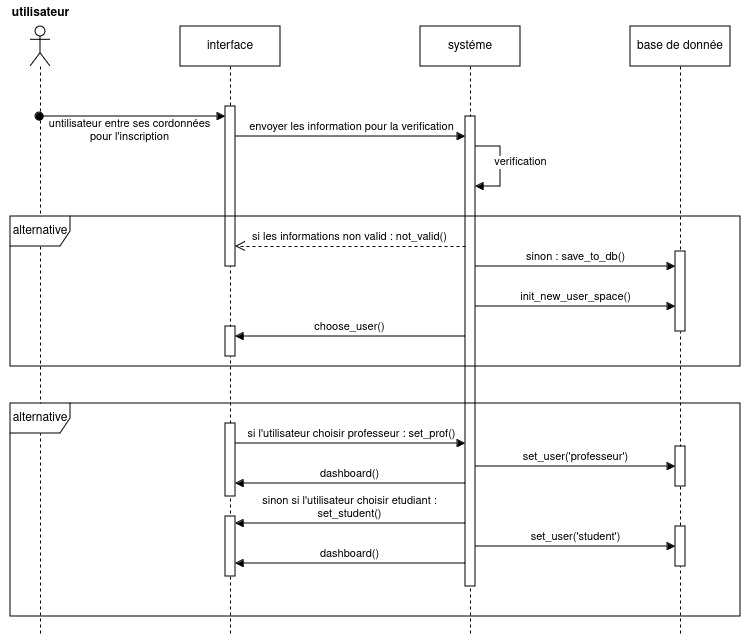
\includegraphics[width=0.65\linewidth]{pages/image/asma-diagramme_sequence-inscription.jpg}
    \caption{Diagramme de séquance  pour l'inscription d'un utilisateur}
    \label{fig:enter-label}
\end{figure}





















\subsection{Réalisation}
Dans cette section on va présenter la réalisation de l'interface pour cette chapitre.
Cette figure représente la page d'acceuil de la plateforme:
\begin{figure}[h!]
    \centering
    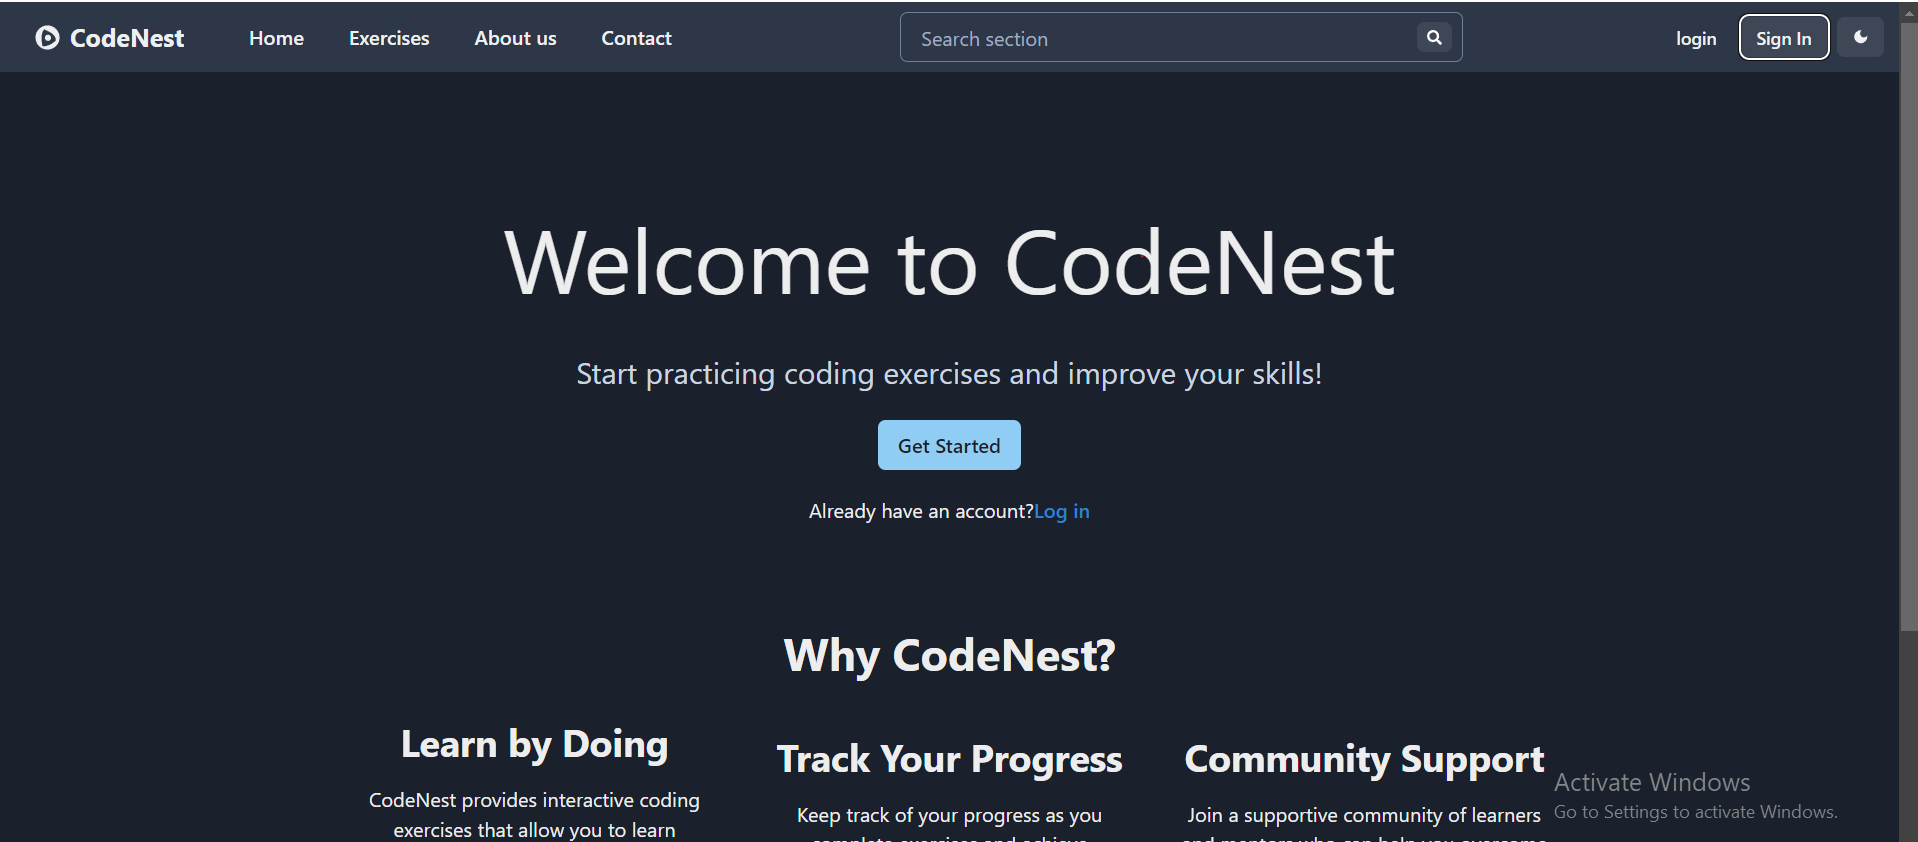
\includegraphics[width=0.9
    \linewidth]{pages/images/interface1.png}
    \caption{Page d'acceuil du plateforme}
    \label{fig:enter-label}
\end{figure}
\\ 



\clearpage 
La figure suivante représante  l'interface du login et sign up  
\begin{figure}[h!]
    \centering
    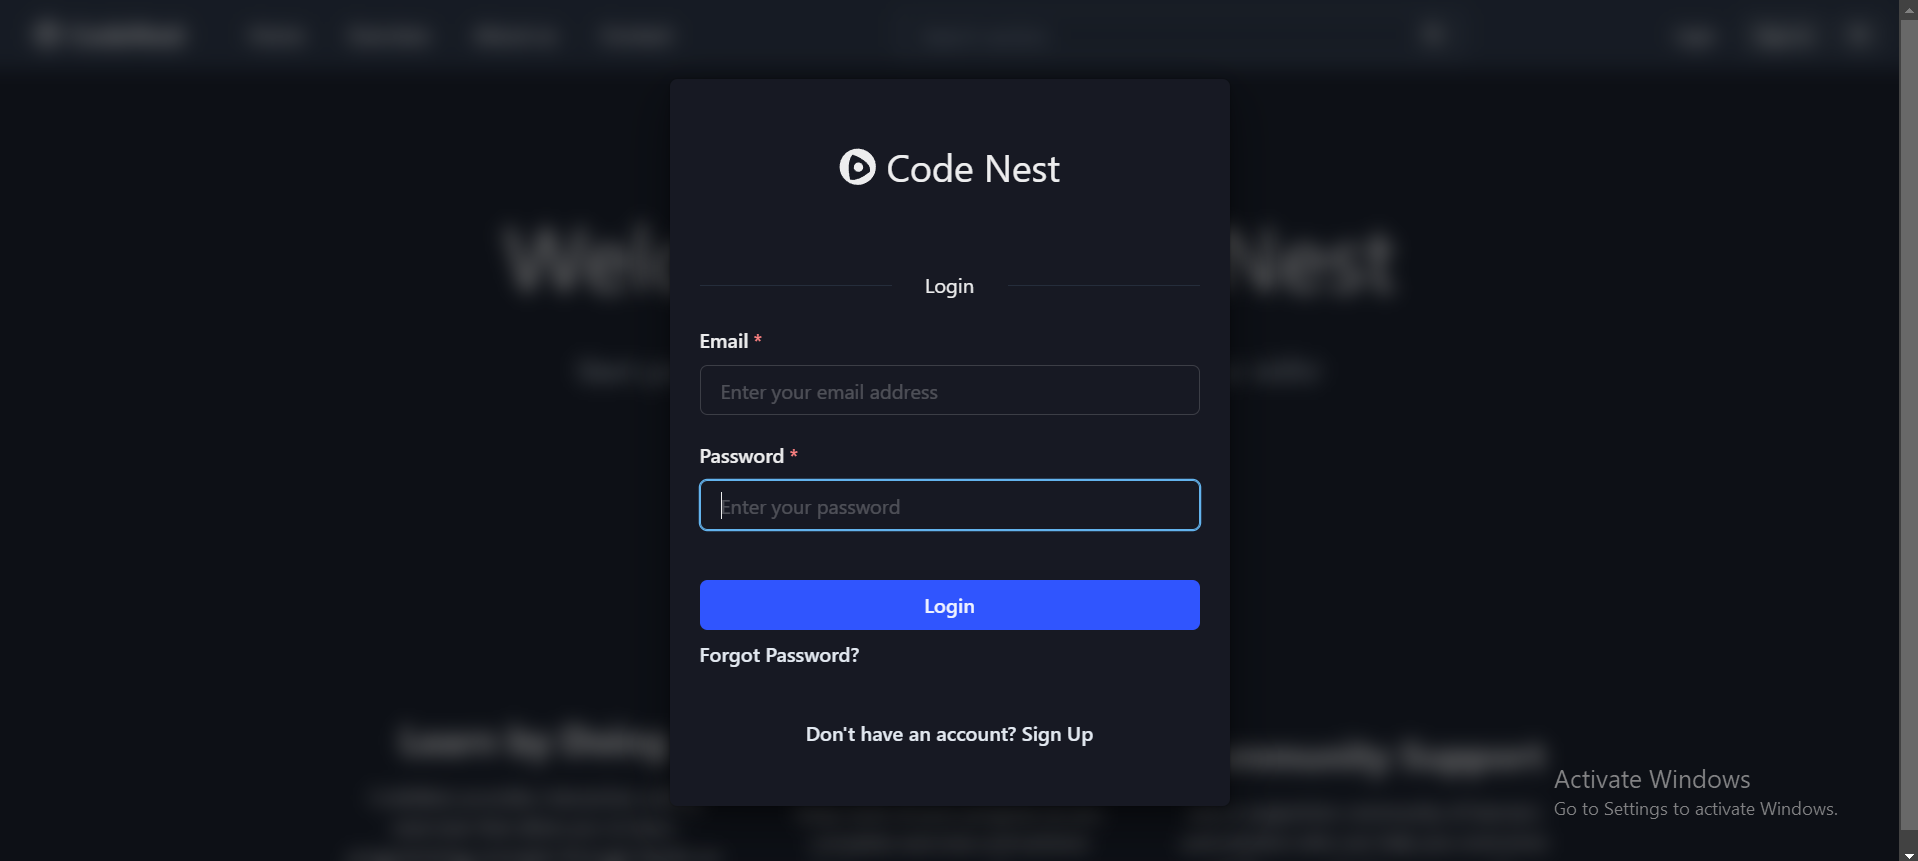
\includegraphics[width=0.9\linewidth]{pages/images/interface login.png}
    \caption{Interface du login du plateforme}
    \label{fig:enter-label}
\end{figure}


\begin{figure}[h!]
    \centering
    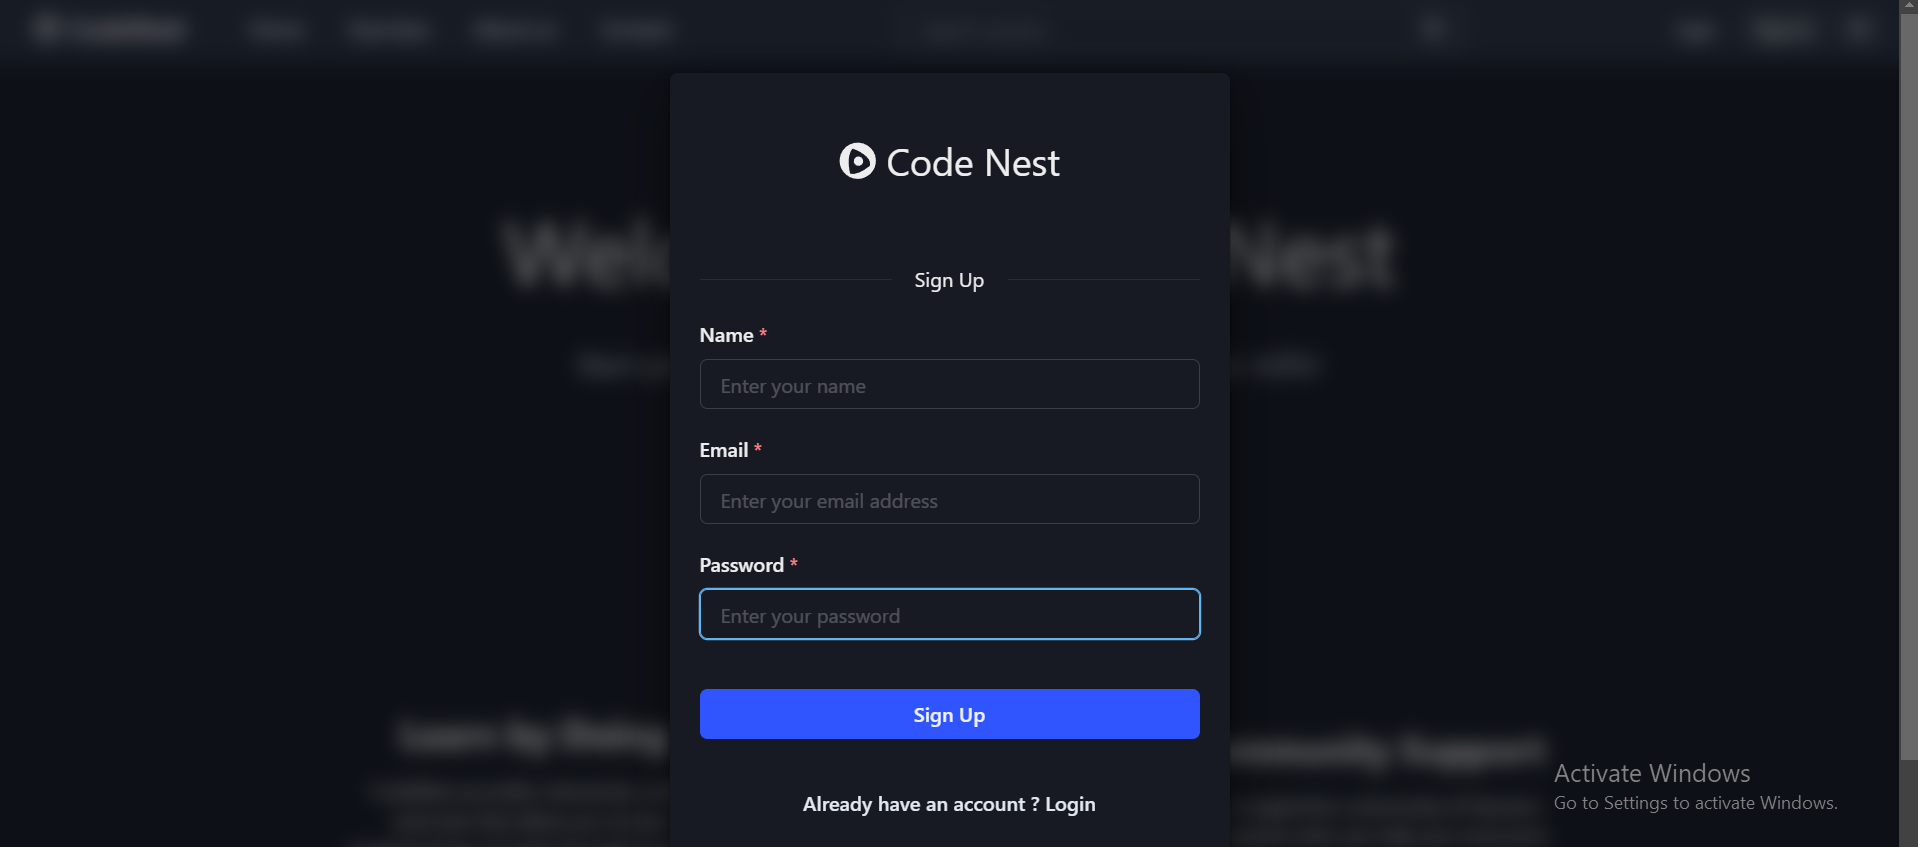
\includegraphics[width=0.9\linewidth]{pages/images/sign up interface.png}
    \caption{Interface de creation de compte du plateforme}
    \label{fig:enter-label}
\end{figure}

\clearpage
La figure montre une interface du compte  d'un utilisateur ou il peut modifier son compte
\begin{figure}[h!]
    \centering
    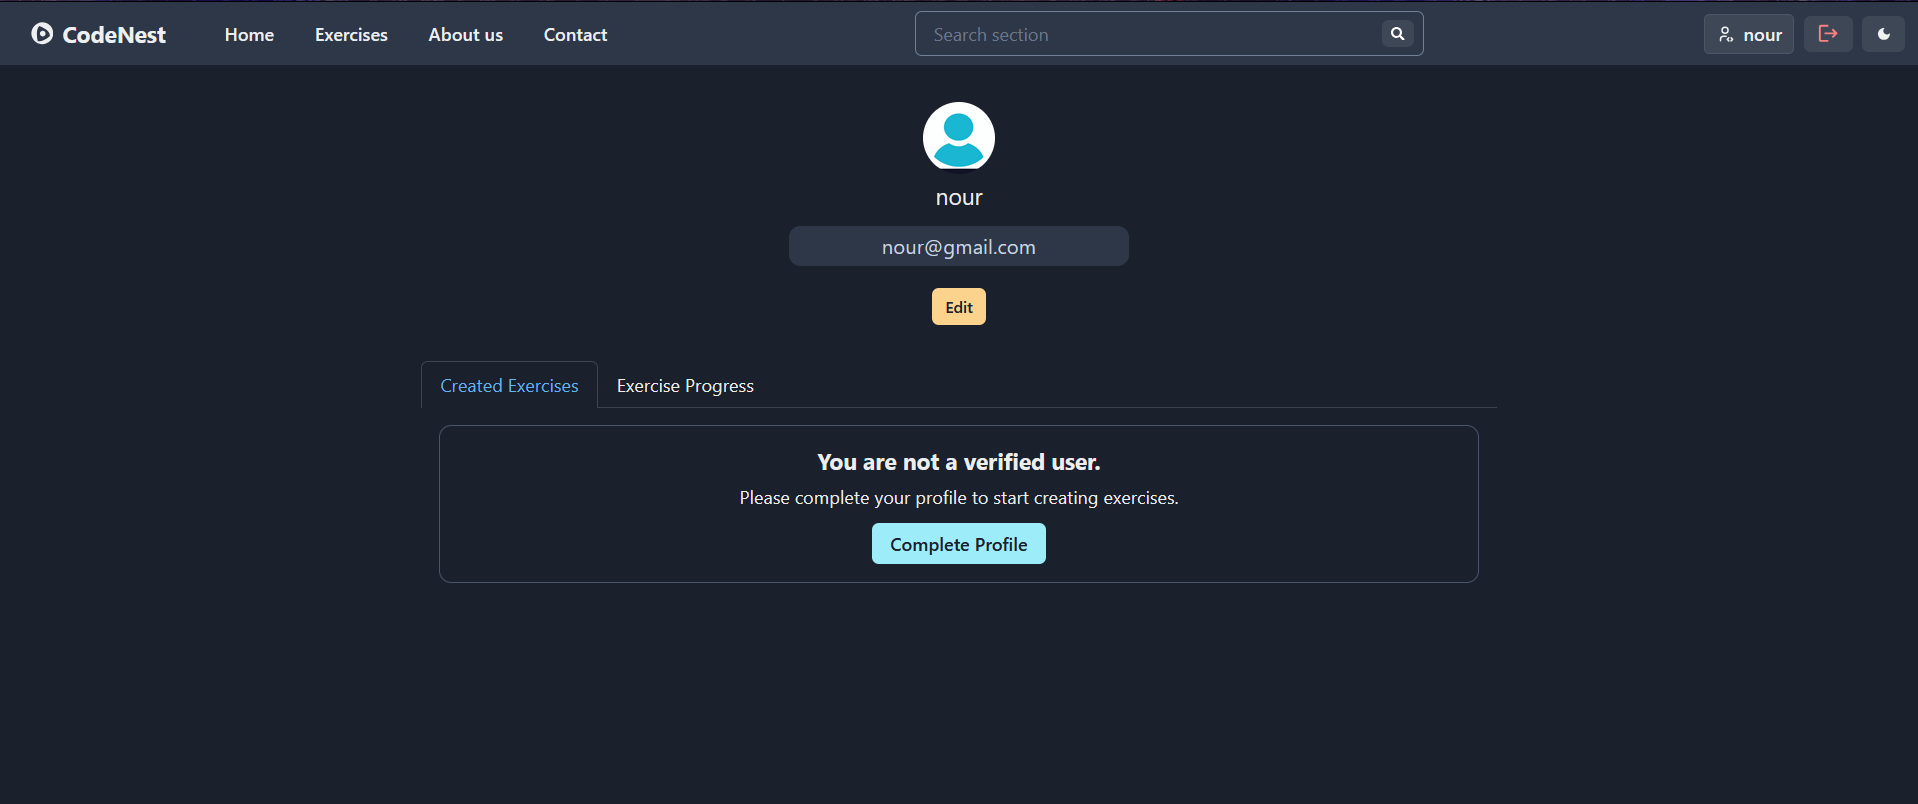
\includegraphics[width=0.9\linewidth]{pages/images/modifier compte.png }
    \caption{Interface utilisateur pour la modification du compte}
    \label{fig:enter-label}
\end{figure}
Au cas d'oublie du mot de passe l'utilisateur peut obtenir un nouveau mot de passe à travérs un email reçu contenant le nouveau code 


\begin{figure}[h!]
    \centering
    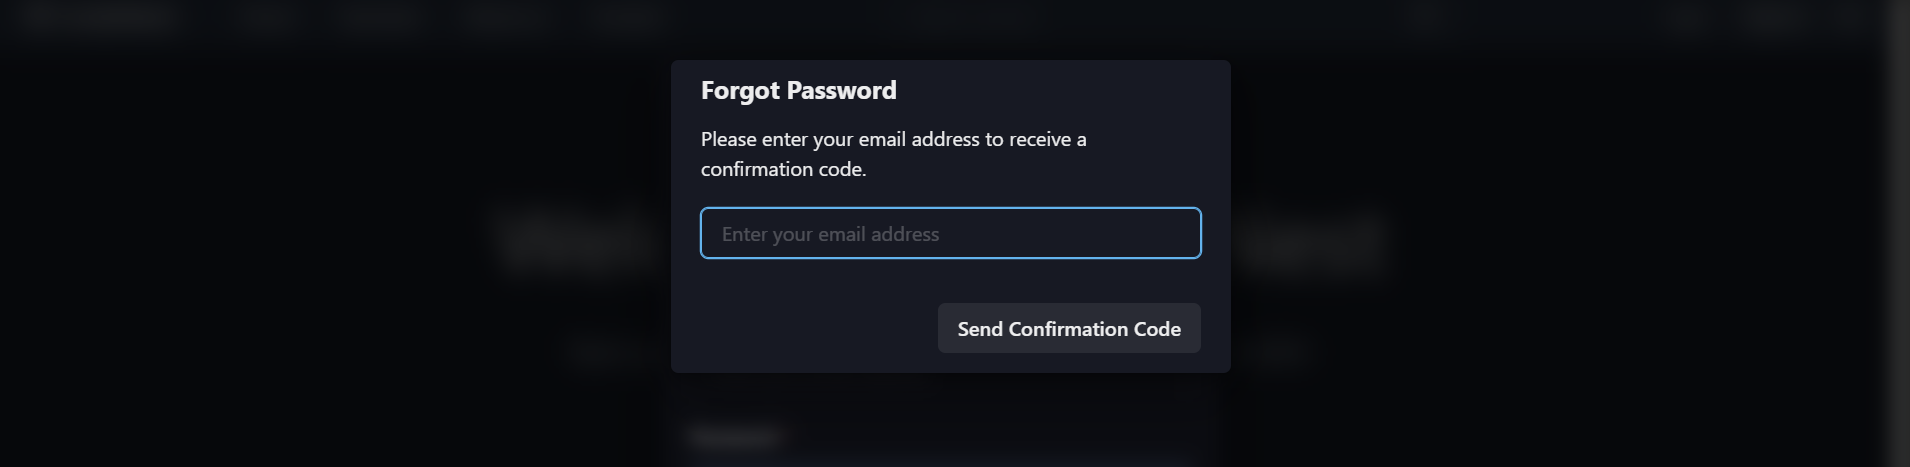
\includegraphics[width=0.9\linewidth]{pages/images/send mail interface.png}
    \caption{Interface utilisateur pour entrer le mail }
    \label{fig:enter-label}
\end{figure}

\begin{figure}[h!]
    \centering
    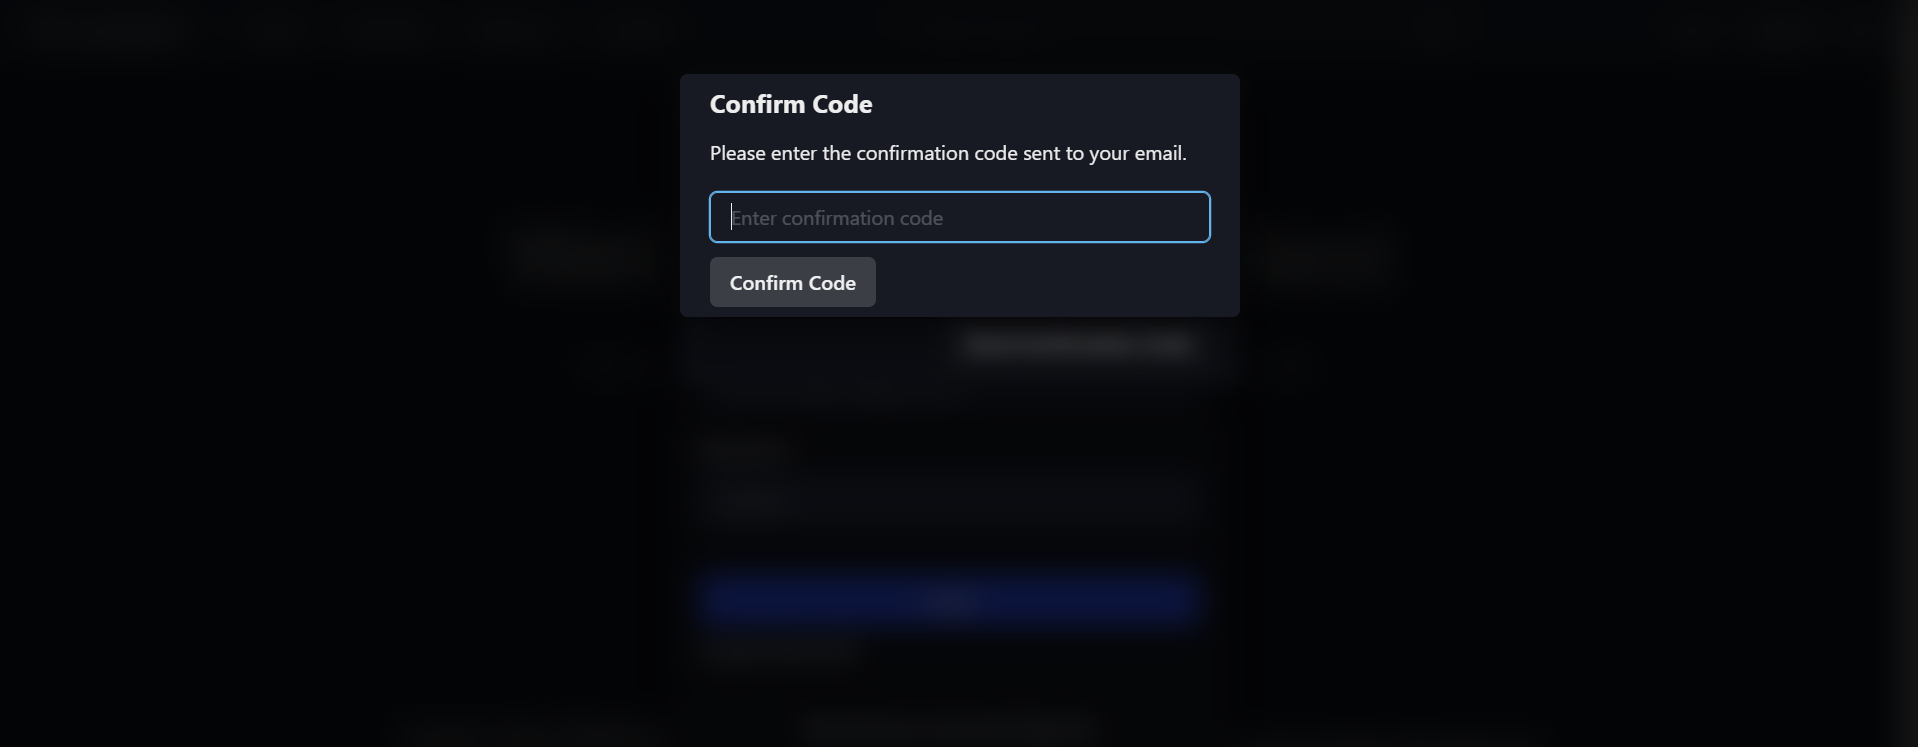
\includegraphics[width=0.9\linewidth]{pages/images/confirmation code interface.png}
    \caption{Interface  l'utilisateur de confirmation du code envoyé sur mail }
    \label{fig:enter-label}
\end{figure}


\clearpage
\section{Conclusion}
Le résultat de notre premier sprint nous permet de rassembler les données utiles pour la prochaine partie du projet. 
A cette étape on est capable de créer un Forum pour notre application web
La prochaine étape sera de traiter le second sprint qui représente une partie importante de note plateforme.